%!TEX encoding = UTF-8 Unicode
\documentclass[12pt]{article} 
\usepackage[left=0.75in,top=0.7in,right=0.75in,bottom=0.3in]{geometry} % Document margins
\usepackage{CJK}
\usepackage{graphicx}
\usepackage{mathtools}
\usepackage{mathrsfs}
\usepackage{amssymb}
\usepackage{hyperref}
\usepackage{sidecap}
\usepackage{makecell}

\makeatletter
\renewenvironment{itemize}
{\list{$\bullet$}{\leftmargin\z@ \labelwidth\z@ \itemindent-\leftmargin
\let\makelabel\descriptionlabel}}
{\endlist}
\makeatother

\begin{CJK}{UTF8}{bsmi}
\title{\textbf{Homework4 / Handwritten Digits Recognition}}
\author{\textbf{李豪韋 (HW-Lee) ID 103061527}}
\date{}

\begin{document}
\vspace*{-60pt}
    {\let\newpage\relax\maketitle}

\section*{Overview}
\vspace{-20pt}
\noindent\makebox[\linewidth]{\rule{\textwidth}{0.4pt}}
\vspace{5pt}

Neural nets can theoretically learn any function, so we can also utilize them to do classification tasks. In recent years, automatic recognition systems have been getting more important and more widely used. Therefore, we try to implement a system that is able to recognize hand-written digits. Obviously, it is a classification problem, all things we have to do are 1) separating instances which belong to different classes as much as possible, 2) aggregating instances which belong to the same class as close as possible, 3) suppressing the confidence of outputs corresponding to wrong classes, and 4) lifting the confidence of the output corresponding to the right class. In this project, the task has been implemented and the average accuracy can achieve close to 90$\%$. The more detailed information of the code is publicly available on \href{https://github.com/HW-Lee/2015-NN-Homeworks/tree/master/HW04}{$\mathsf{https://github.com/HW}$-$\mathsf{Lee/2015}$-$\mathsf{NN}$-$\mathsf{Homeworks/tree/master/HW04}$}.

\section*{Implementation}
\vspace{-20pt}
\noindent\makebox[\linewidth]{\rule{\textwidth}{0.4pt}}

\begin{enumerate}
	\item {\bf Net Structure}
	\begin{SCfigure}[][h]
		\hspace*{-2em}
		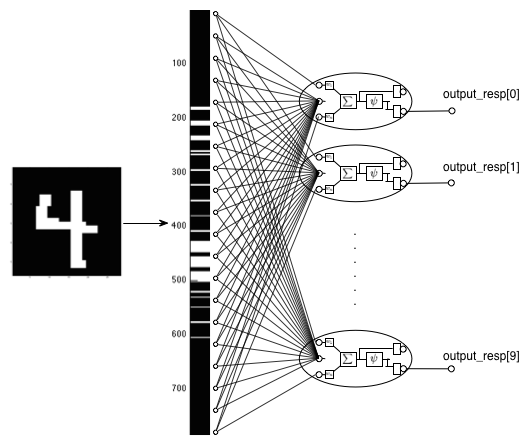
\includegraphics[scale=.65]{../res/netStruct.png}
		\caption{The structure of net. It simply consists of 10 neurons without any hidden unit, which acts like a linear filter, and the image data will be reshaped from 2D to 1D then all pixels will be regarded as an input port. However, the only thing different from the linear filter implemented in Hw2 is that the linear outputs are cascaded to the logistic function that maps any real value into a value ranged from 0 to 1, in order to make the output a measure of 'confidence'. Finally, the prediction is followed by the rule of choosing the class which turns out the highest confidence.}
	\end{SCfigure}
	
	\newpage
	\item {\bf Process}
	\begin{itemize}
		\item {\bf Weights Initialization}: make an initial guess.
		\item {\bf Randomly Feeding Instances}: randomly choose an instance with its ground truth.
		\item {\bf Stochastic Gradient Descent}: Use SGD to obtain a good set of weights.
	\end{itemize}
\end{enumerate}

\section*{Results}
\vspace{-20pt}
\noindent\makebox[\linewidth]{\rule{\textwidth}{0.4pt}}

\begin{enumerate}
	\item {\bf Confusion matrix with cross-validation (average accuracy is 0.877)}
	\begin{center}
	\begin{tabular}{|c|c|c|c|c|c|c|c|c|c|c|}
		\hline
		\diaghead{\theadfont Diag ColumnmnHead II}{truth}{result} 
		& '0' & '1' & '2' & '3' & '4' & '5' & '6' & '7' & '8' & '9' \\
		\hline
		'0' & {\bf 0.99} & 0.00 & 0.00 & 0.00 & 0.00 & 0.00 & 0.00 & 0.00 & 0.01 & 0.00 \\ 
		\hline
		'1' & 0.00 & {\bf 0.94} & 0.02 & 0.00 & 0.00 & 0.02 & 0.00 & 0.00 & 0.02 & 0.00 \\ 
		\hline
		'2' & 0.01 & 0.01 & {\bf 0.87} & 0.00 & 0.01 & 0.00 & 0.01 & 0.03 & 0.05 & 0.01 \\ 
		\hline
		'3' & 0.01 & 0.00 & 0.04 & {\bf 0.84} & 0.01 & 0.04 & 0.02 & 0.03 & 0.01 & 0.00 \\ 
		\hline
		'4' & 0.00 & 0.01 & 0.03 & 0.01 & {\bf 0.85} & 0.01 & 0.02 & 0.03 & 0.02 & 0.02 \\ 
		\hline
		'5' & 0.05 & 0.00 & 0.00 & 0.07 & 0.03 & {\bf 0.79} & 0.01 & 0.00 & 0.04 & 0.01 \\ 
		\hline
		'6' & 0.00 & 0.00 & 0.00 & 0.01 & 0.01 & 0.03 & {\bf 0.94} & 0.00 & 0.01 & 0.00 \\ 
		\hline
		'7' & 0.01 & 0.01 & 0.01 & 0.00 & 0.01 & 0.00 & 0.00 & {\bf 0.93} & 0.00 & 0.03 \\ 
		\hline
		'8' & 0.01 & 0.03 & 0.01 & 0.04 & 0.01 & 0.00 & 0.01 & 0.02 & {\bf 0.85} & 0.02 \\ 
		\hline
		'9' & 0.04 & 0.02 & 0.01 & 0.02 & 0.06 & 0.02 & 0.01 & 0.04 & 0.01 & {\bf 0.77} \\ 
		\hline
	\end{tabular}
	\end{center}
	
	\item {\bf Confusion matrix with empirical data (average accuracy is 0.9124)}
	\begin{center}
	\begin{tabular}{|c|c|c|c|c|c|c|c|c|c|c|}
		\hline
		\diaghead{\theadfont Diag ColumnmnHead II}{truth}{result} 
		& '0' & '1' & '2' & '3' & '4' & '5' & '6' & '7' & '8' & '9' \\
		\hline
		'0' & {\bf 0.98} & 0.00 & 0.00 & 0.00 & 0.00 & 0.00 & 0.00 & 0.00 & 0.00 & 0.00 \\ 
 		\hline 
		'1' & 0.00 & {\bf 0.96} & 0.01 & 0.00 & 0.00 & 0.01 & 0.00 & 0.00 & 0.01 & 0.00 \\ 
 		\hline 
		'2' & 0.01 & 0.01 & {\bf 0.87} & 0.01 & 0.02 & 0.00 & 0.02 & 0.02 & 0.02 & 0.01 \\ 
 		\hline 
		'3' & 0.00 & 0.01 & 0.03 & {\bf 0.87} & 0.00 & 0.03 & 0.01 & 0.01 & 0.01 & 0.02 \\ 
 		\hline 
		'4' & 0.00 & 0.01 & 0.00 & 0.00 & {\bf 0.92} & 0.00 & 0.01 & 0.00 & 0.00 & 0.04 \\ 
 		\hline 
		'5' & 0.02 & 0.01 & 0.01 & 0.03 & 0.01 & {\bf 0.86} & 0.02 & 0.00 & 0.03 & 0.01 \\ 
 		\hline 
		'6' & 0.01 & 0.00 & 0.00 & 0.00 & 0.00 & 0.01 & {\bf 0.97} & 0.00 & 0.00 & 0.00 \\ 
 		\hline 
		'7' & 0.01 & 0.01 & 0.01 & 0.00 & 0.02 & 0.00 & 0.00 & {\bf 0.93} & 0.00 & 0.02 \\ 
 		\hline 
		'8' & 0.01 & 0.01 & 0.02 & 0.02 & 0.01 & 0.02 & 0.02 & 0.01 & {\bf 0.88} & 0.01 \\ 
 		\hline 
		'9' & 0.02 & 0.00 & 0.01 & 0.02 & 0.02 & 0.01 & 0.00 & 0.04 & 0.00 & {\bf 0.89 } \\ 
 		\hline 
	\end{tabular}
	\end{center}
	
	\newpage
	\item {\bf Average response with different classes}
	\begin{figure}[ht]
		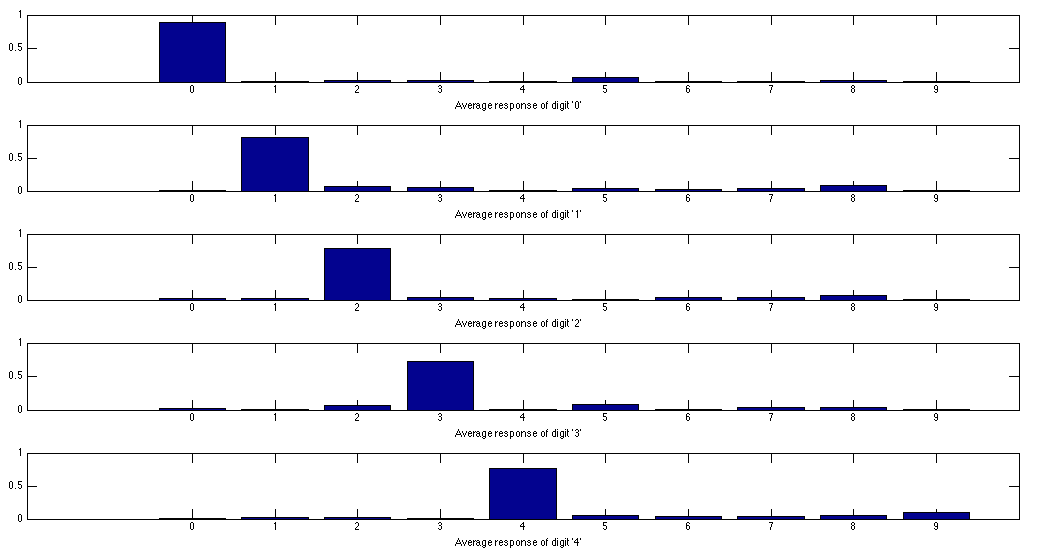
\includegraphics[scale=.5]{../res/resp0-4.png}
		\vspace*{-2em}
	\end{figure}
	\begin{figure}[ht]
		\vspace*{-2em}
		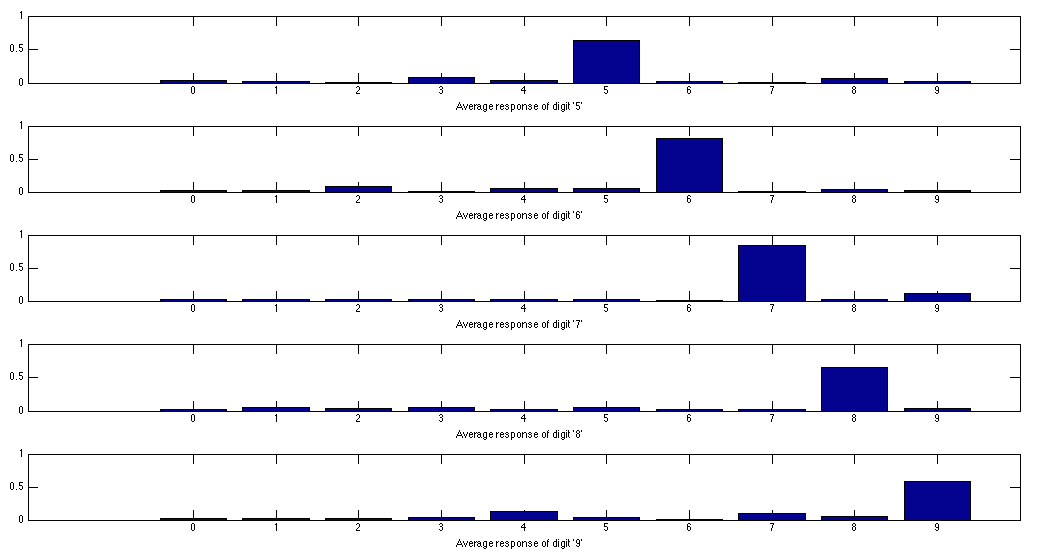
\includegraphics[scale=.5]{../res/resp5-9.png}
		\caption{the response evaluated with 100 randomly sampled images of each class}
		\vspace*{-2em}
	\end{figure}
\end{enumerate}


\newpage
\section*{Discussion}
\vspace{-20pt}
\noindent\makebox[\linewidth]{\rule{\textwidth}{0.4pt}}

\begin{enumerate}
	\item What is a good initialization strategy?
	\begin{flushleft}
		Actually, any initialization method will not affect the performance too much because the structure of my system is not complex, most of issues concerned in back-propagation applied to multi-layer net are not critical in gradient descent of linear filters (e.g. no zero-initialization, random variation). However, an appropriate initial guess will decrease lots of computation time for learning with training sets. In practice, a system with better initial weights gets converged after 30,000 iterations while that with randomly initialized weights gets converged after more than 100,000 iterations. Then, what is a good set of initial weights? I use the training strategy described in the homework description sheet, namely simply averaging all training data of each class, I use it as the initial weights. It is a good initial guess such that the system can get converged only with 30,000 iterations!
	\end{flushleft}
	\item How to define input space?
	\begin{flushleft}
		As the sheet described, every image only contains raw data with value either 0 or 1. If we only apply it as the input space directly, the offset(0) can not be used as a 'penalty' while training. (because the value 0 is constant with any arbitrary weight) For enabling the sensitivity of offset, the data are subtracted by 0.5 for the purpose of making data ranged in $\pm 0.5$. Hence, the offset is as sensitive as the onset and the input space is balanced. (0-centred range)
	\end{flushleft}
	\item Something interesting of final weights.
	\begin{figure}[ht]
		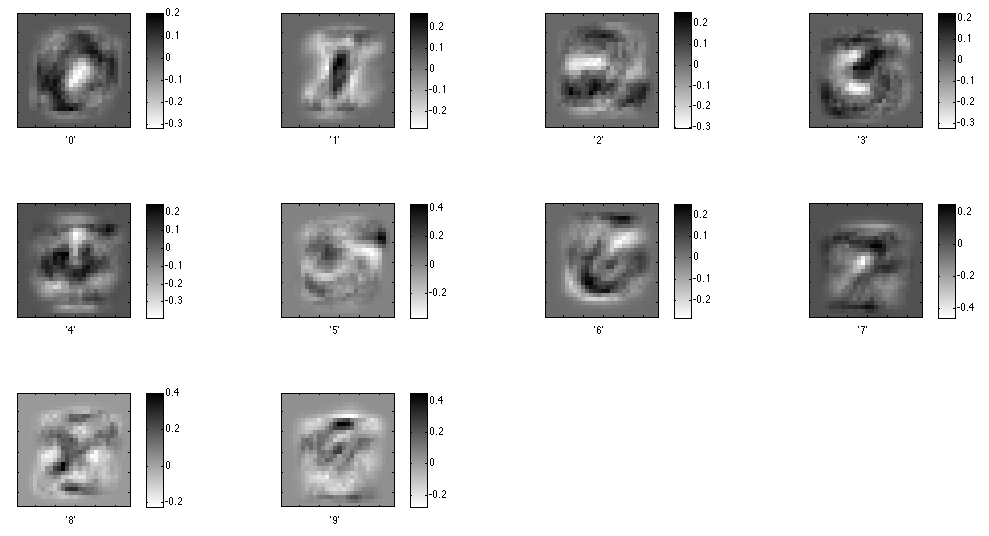
\includegraphics[scale=.5]{../res/weights2D.png}
		\vspace*{-1em}
		\caption{Final weights reshaped to 2D (with the same structure as that of images) of each class. There comes some intuitive and interesting conclusions: 1) The final weights get converged to the results which are 'visually similar' to the appearance of digits we think. 2) The brighter parts, which refers to relatively smaller values, in each class are also features that people use to recognize a digit. (e.g. we expect that there is a 'hole' at the center of '0', and there are two vertically arranged holes in '8'.)}
		\vspace*{-5em}
	\end{figure}
\end{enumerate}

\end{CJK}
\end{document}